\subsection*{Projektplan}

\begin{figure}[h]
    \centering
    \begin{minipage}[b]{\textwidth}
        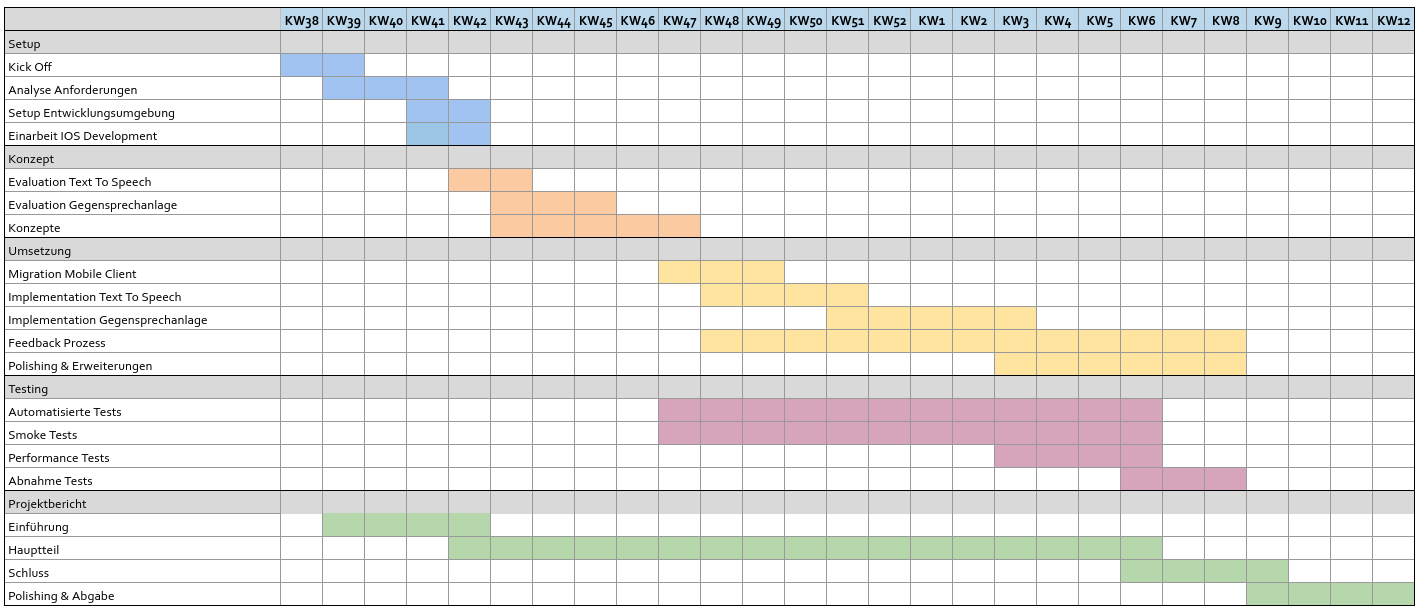
\includegraphics[width=\textwidth]{graphics/projektplan}
        \caption{Projektplan}
    \end{minipage}\label{fig:projektplan}
\end{figure}

In der ersten Phase des Projektes (KW38-KW42) wird das Projekt aufgesetzt.
Anforderungen und Umfang des Projektes werden zusammen mit dem Auftraggeber erarbeitet und anschliessend dokumentiert.
Es wird ein Projektplan erstellt und die ersten Teile des Projektberichts werden aufgesetzt.
Infrastruktur und Codebasis des Vorgängerprojektes wird übernommen und wo nötig für dieses Projekt angepasst.
Für die Entwicklung des nativen Mobile Clients muss die Entwicklungsumgebung inklusive Apple Hardware aufgesetzt werden.
Während dieser Zeit arbeitet sich das Projektteam bereits in die iOS Entwicklung ein um erste Erfahrungen zu sammeln und um zu validieren, dass die Entwicklungsumgebung vollständig und funktionsfähig ist.
In der zweiten Phase (KW42-KW47) werden primär Konzepte erarbeitet und validiert.
Dies beinhaltet das evaluieren von Technologien, das definieren und dokumentieren von Grundprozessen und Datenstrukturen.
Die erstellten Konzepte sollen mit möglichst einfachen Proof Of Concepts validiert werden.
Weiter wird dokumentiert, wie die bestehende Systemarchitektur erweitert wird um die neuen Funktionen zu ermöglichen.
Dabei müssen insbesondere Skalierbarkeit, Erweiterbarkeit und Integrierbarkeit des Systems bewahrt werden.
Die Umsetzung des Systems findet schliesslich in der dritten Pase (KW47-KW08) statt.
Die festgehaltenen Anforderungen und Konzepte werden implementiert.
Dabei wird as erstes der bestehende Mobile Client neu in eine native iOS Applikation migriert.
Darauf wird der Client um die Sprachsynthesefunktion und letztlich um die Funktion Gegensprechanalge erweitert.
Die erarbeiteten Konzepte werden in dieser Phase laufend überarbeitet und angepasst.
Sobald die Applikation einen gewissen Reifegrad erreicht hat, soll der Kunde mittesten und Input geben können, welche Änderungen und Erweiterungen er wünscht.
Diese werden soweit es der zeitliche Rahmen erlaubt mit eingearbeitet.
Während der Umsetzung werden laufend automatisierte Tests geschrieben und Smoketests durchgeführt.
Zum Ende der Umsetzungsphase sollen zudem Performance Metriken erfasst werden.
Als letzter Test wird schliesslich ein Abnahmetest mit dem Kunden durchgeführt.
Die vierte Phase (KW09-KW12) bildet den Abschluss des Projekts.
Es werden keine Änderungen mehr an der Applikation vorgenommen.
Der Projektbericht wird fertiggestellt und das Projekt wird für die Abgabe vorbereitet.

\clearpage
